% !TeX root = ./PhDThesis.tex

\chapter{Cryogenic experimental techniques}
\label{chap:cryogenic_experimental_techniques}

\section{Cool-down and warm-up procedures}

The cryogenic trapped-ion system is a relatively complex experimental system, and we need the system to be stable over a long period of time so that the reproducibility of the measurement results is high. Although the cryostat's core component, the cold head, can run continuously for more than 10,000 hours, the maximum time this cryostat can run continuously is limited by the stability of the power supply, the stability of the laboratory temperature and humidity, and whether the exchange gas space is leaking, as shown in Fig~\ref{fig:fig_4_exchange_gas_space_leakage}. It took us about three years to get the system into a stable long-term state, after which we conducted a series of physical experiments on the experimental platform. However, during the three-year commissioning process, we inevitably need to conduct the cycle of cool-down, malfunction, warm-up, and upgrade, during which the standardized operation helps to make the physical parameters of the system more repeatable, so we have developed a standardized operation procedure for this system.

\subsection{Maintenance of the exchange gas space}
If the cold head does not need to be removed for servicing, the exchange gas space does not require frequent maintenance and is always in an independent and stable state, whether it is being cooled down or warmed up.

The exchange gas space uses helium gas with a purity of 99.999\%. When we expose the exchange gas space to atmosphere or when it is first used, the internal gas needs to be purified. According to the cryostat manufacturer's recommendations, a purification is also required after several months of continuous running, but this is not normally done when the system is stable for a long period of time. How often the exchange gas space needs to be purified depends on the rate of impurity gases (nitrogen, oxygen, water vapour etc.) leaking in from the atmosphere.

When we need to purify the helium gas in the exchange gas space, the exchange gas space is first evacuated continuously for 0.5 hours with a dry scroll pump (Agilent IDP-7), then the valve connected to the dry scroll pump is closed and the valve connected to the helium gas is opened. The auto gas charging system will then raise the pressure to 1.03 bar and finally we close the valve to the helium gas. In general, the above operation is repeated three times to purify the helium gas in the exchange gas space.

\begin{figure}
    \centering
    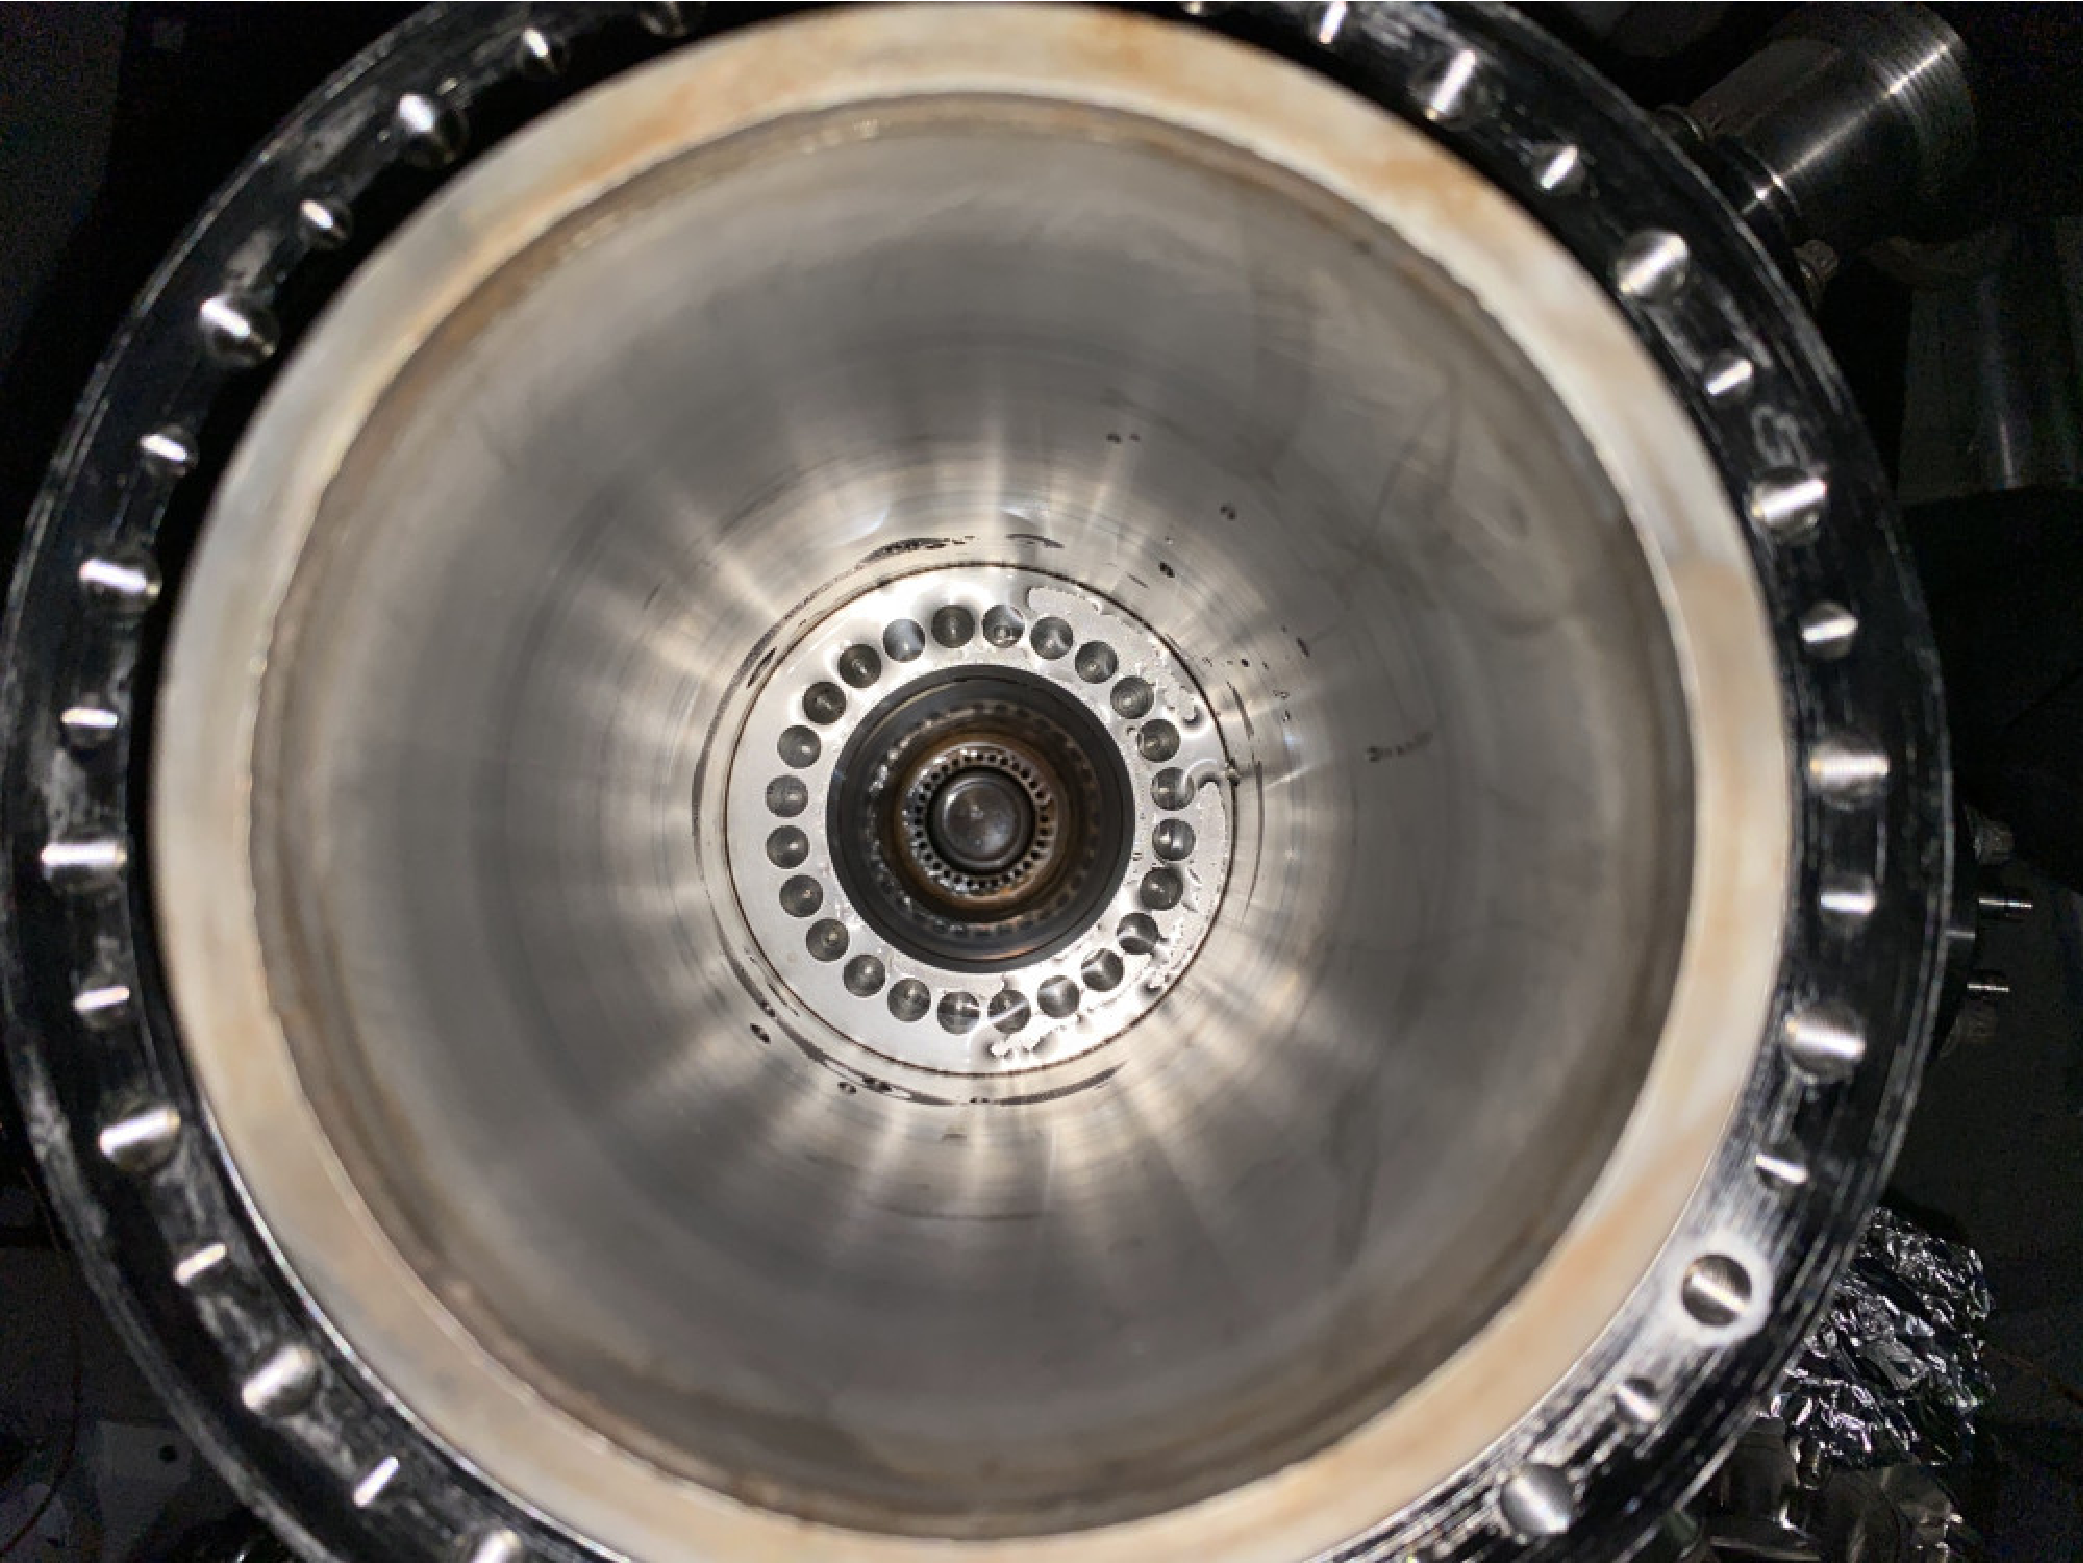
\includegraphics[width=0.8\linewidth]{fig_4_exchange_gas_space_leakage.pdf}
    \caption{Observation of leakage in the exchange gas space.}
    \label{fig:fig_4_exchange_gas_space_leakage}
\end{figure}

When we need to cool down or warm up the system, and also when the system is running at low temperatures for a long time, we simply open the valve to the helium gas and keep the auto gas charging system running steadily.

\subsection{Cool-down}

In the cool-down procedure, the physical parameters of the vacuum chamber are mainly adjusted and observed. The vacuum chamber is first connected to a turbo-molecular pump (TPS-compact Turbo Pumping System) via the angle valve and after approximately 48 hours of continuous operation the vacuum chamber reaches a vacuum level close to UHV. The ion gauge is switched on and reaches an indication of $5 \times {10}^{-8}$ mbar, at which point we do not need to degas the ion gauge as the room temperature zone of the vacuum chamber does not eventually fall below $1 \times {10}^{-10}$ mbar. Now we need to perform a time limited activation of the NEG Pump for 1 hour, then we perform several degas of the Ion Pump and keep the Ion Pump on. Now that the activation of the NEG-Ion Pump is complete, we close the angle valve and wait about 1 hour for the ion gauge to gradually decrease to $3 \times {10}^{-9}$ mbar, when the vacuum chamber reaches the UHV vacuum level. We turn on the cold head and the temperature stabilize system, which will finish cooling down within 5 hours, but the system will not reach final stabilization for more than 24 hours. The temperature of the 4 K stage is finally stabilised at 6 K and the ion gauge is stabilised at $3 \times {10}^{-10}$ mbar.

\begin{figure}
    \centering
    \subcaptionbox{Temperature vs. time.}
    {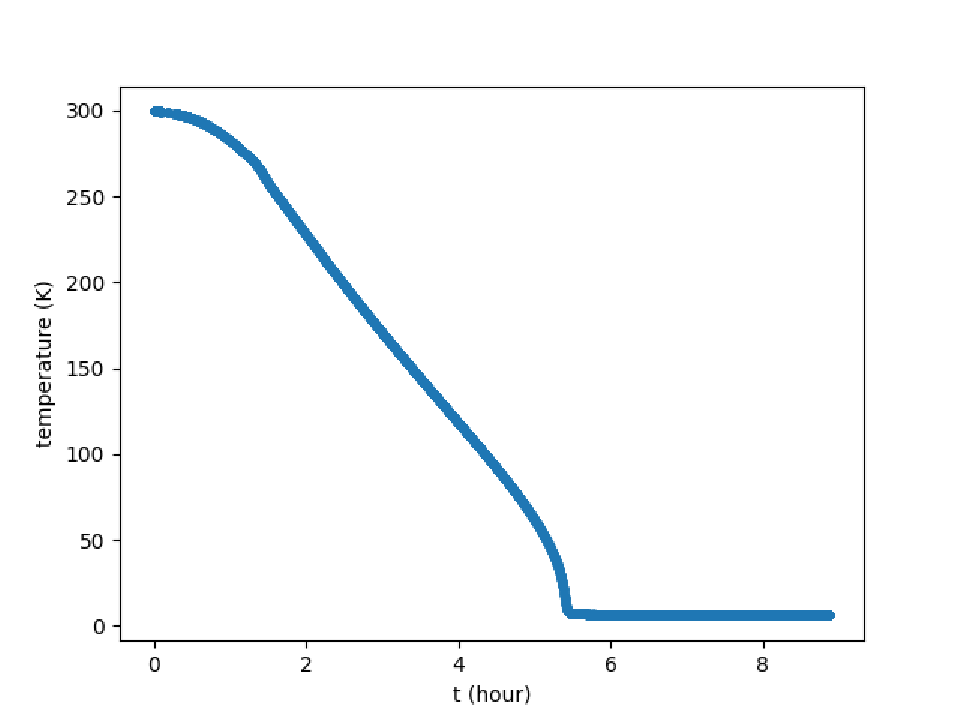
\includegraphics[width=0.4\linewidth]{fig_4_cool_down_temperature.pdf}}
    \subcaptionbox{Pressure vs. time.}
    {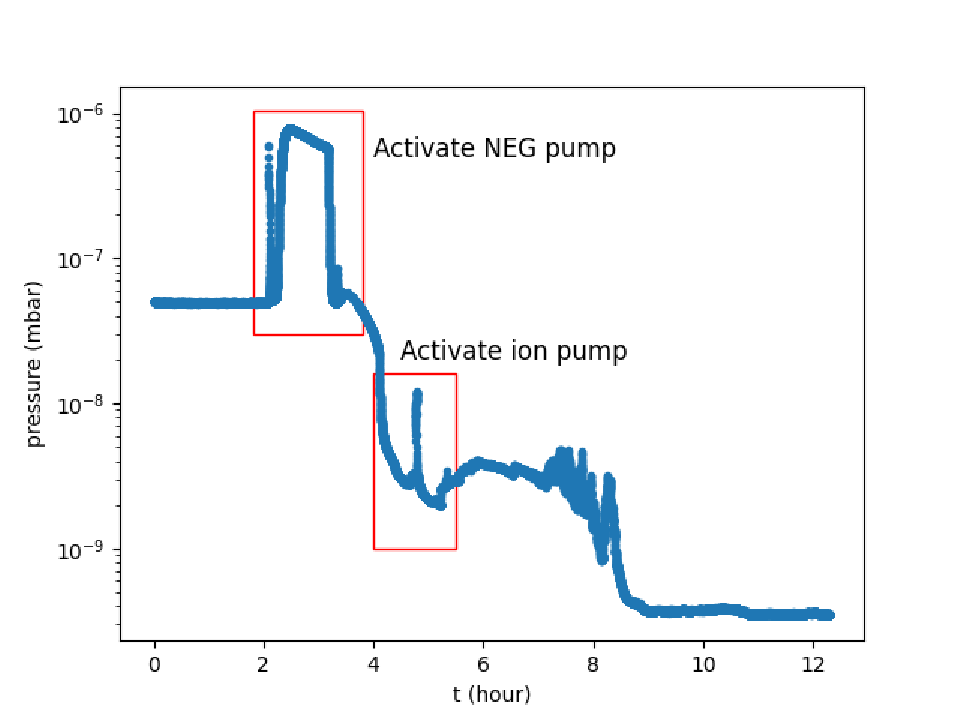
\includegraphics[width=0.4\linewidth]{fig_4_cool_down_pressure.pdf}}
    \caption{Cryostat temperature and pressure over time during a cool-down.}
\end{figure}

\subsection{Warm-up}

The warm-up procedure is much easier than the cool-down procedure because we do not need to obtain UHV during this process. we turn off the cryogenic and vacuum related instruments: the NEG-Ion pump, the ion gauge, the cold head. We can use the heater in the temperature stabilize system to heat the cryostat to speed up the warming process to room temperature, which takes about 24 hours or more \cite{RN357}. The system can also be allowed to warm up naturally to room temperature, which takes about 48 hours or more. Next, if necessary, we can move the cryostat into the service area for servicing. Before moving it out, we need to record the readings of all optical and electrical instruments. As the imaging system is embedded in the re-entrant window, we usually need to remove the objective lens.

\begin{figure}
    \centering
    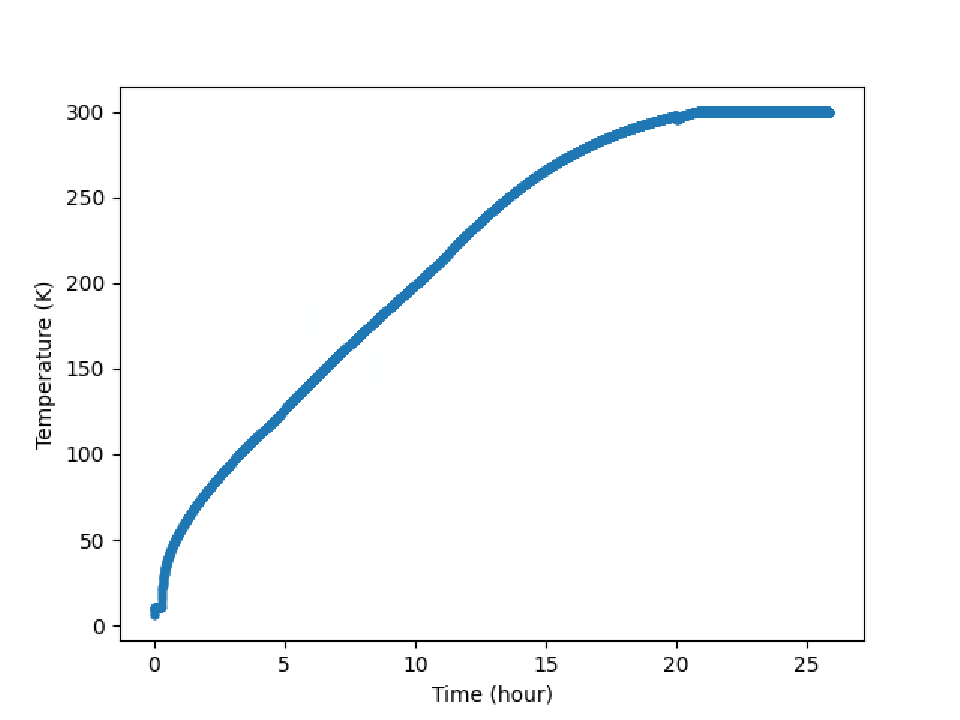
\includegraphics[width=0.4\linewidth]{fig_4_warm_up_temperature.pdf}
    \caption{Cryostat temperature over time during a warm-up.}
\end{figure}

\section{Characterization of the vibration}

A stimulated two-photon Raman process using a pulsed 355 nm laser is used to produce the spin-spin interactions. Because of this, any displacement of the ion chain that occurred during the contact period that was on the order of the wavelength of the Raman laser would create an undesirable phase shift in the ions. As a result, it is of the most importance to minimize the vibration that occurs inside this Gifford-McMahon closed-cycle cryostat \cite{RN126}.

\subsection{The Michelson interferometer}

Although there are many different instruments for measuring vibration signals, such as capacitive sensors for vibration measurement, most of them are not suitable for use in our systems. Measurement of vibration signals in UHV systems at cryogenic temperatures is mainly done by non-contact measurement, and the use of lasers is a very good solution for non-contact measurement, which is also suitable for our systems. There are two main solutions for measuring position information based on laser, the laser Doppler vibrometer and the laser interferometer \cite{RN295}. The laser Doppler vibrometer measures the spectrum of vibration signals mainly according to the Doppler principle. Its measurement accuracy is dependent on the speed of the object's movement and is therefore very accurate for high frequency signals. However, the cryostat vibration signal does not generally exceed 200 Hz. We are concerned on the one hand with vibration signals that may change the relative phase between the ion and the laser during the laser manipulation sequence, which can usually be measured on the cryostat at frequencies between 10 Hz and 200 Hz and amplitudes between 1 nm and 100 nm. In this frequency range, the laser Doppler vibrometer is not very accurate. On the other hand, we are concerned with the displacement of the trap relative to the optical path over a long experimental period, e.g. one hour. The accuracy of the laser Doppler vibrometer in measuring this long term drift is very low, typically measured with an error of no less than 100 nm, mainly due to the fact that most laser Doppler vibrometers use a velocity integration method to calculate the displacement.

\begin{figure}
    \centering
    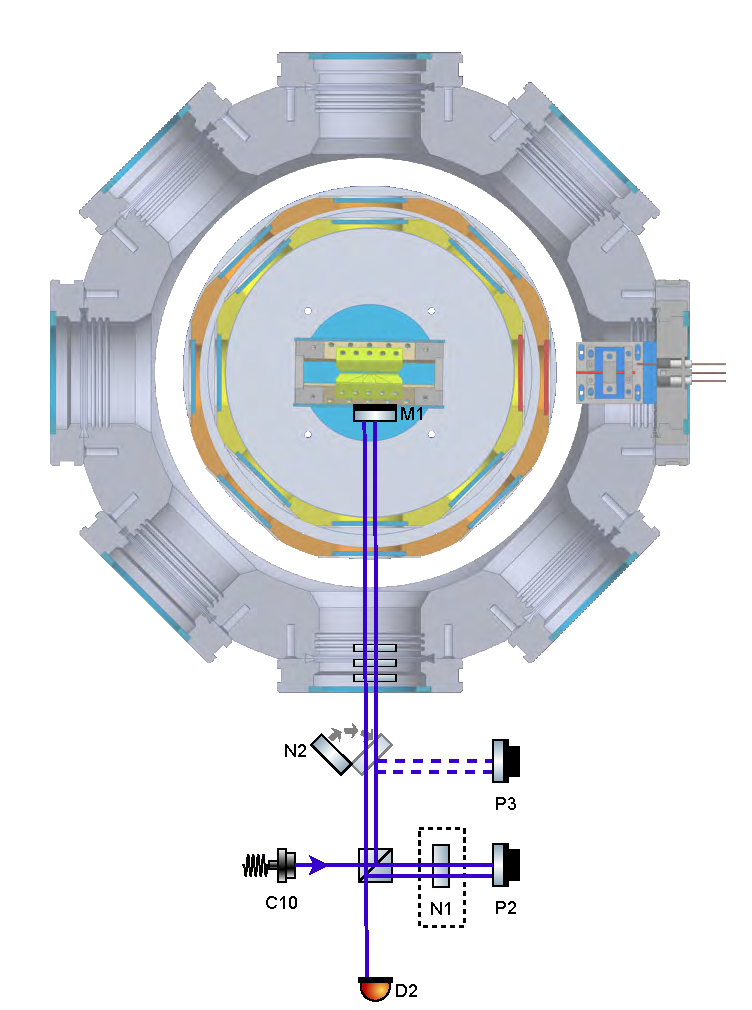
\includegraphics[width=0.8\linewidth]{fig_3_optical_path_370_Interferometer.pdf}
    \caption{Optical layout of the Michelson interferometer.}
    \label{fig:fig_3_optical_path_370_Interferometer}
\end{figure}

The laser interferometer is one of those instruments that is commonly used for measuring displacement and its principle and performance meet our requirements for vibration measurement. Unlike the more industrially used dual-frequency laser interferometer, I have built a very simple Michelson interferometer in my laboratory, as shown in Fig~\ref{fig:fig_3_optical_path_370_Interferometer}, because commercially available laser interferometers are generally not compatible with ultra-high vacuum systems and are not suitable for use in very compact chambers.

\begin{figure}
    \centering
    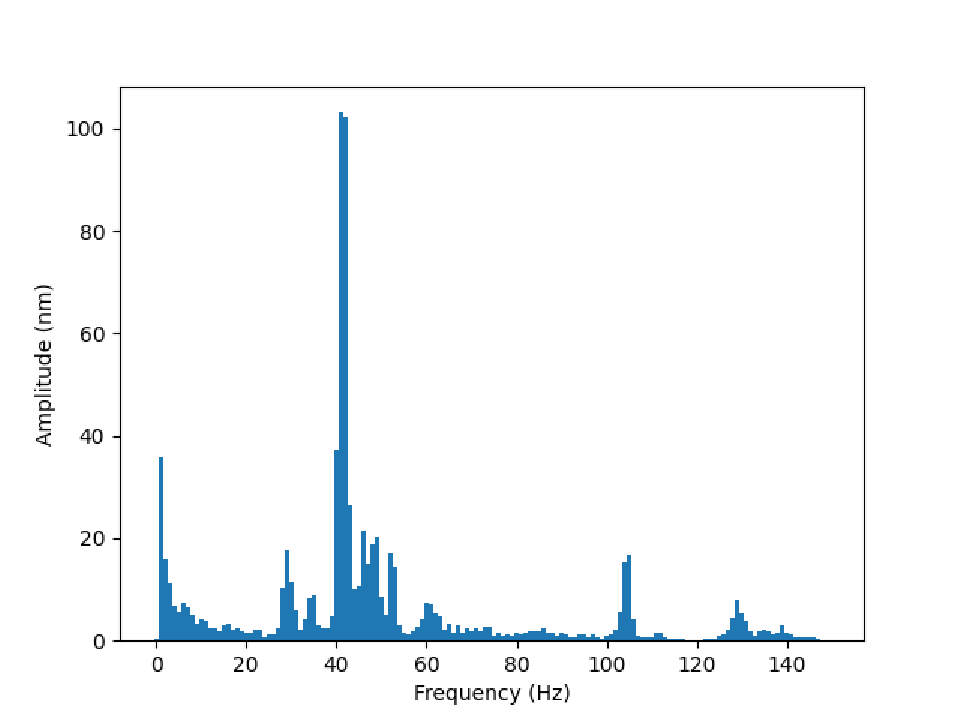
\includegraphics[width=0.8\linewidth]{fig_4_vibration_S302.pdf}
    \caption{Vibration in the horizontal plane of this cryostat.}
\end{figure}

Experimentally we will fix a small reflector (M1), about 6 mm in diameter, to the trap holder, which is located in the 4 K reigon inside the cryostat. We have tried using silver epoxy to hold the mirror to the trap holder, but usually the epoxy is detrimental to our ability to obtain XHV and it would be better to use UHV compatible plastic screws to hold the mirror in place. Since it is so well fixed, we believe that the trap displacement can be calculated by measuring the change in the relative optical path of the reflector. The laser is emitted from outside the chamber and then returned from inside the chamnber through six transmissions and one reflection from the reflector, 4 K shield glass, 40 K shield glass and the viewport of the vacuum chamber. Therefore, it is often necessary to place an optical coating on the surface of these glasses to increase the transmission and reflectivity and thus improve the signal-to-noise ratio of the interferometric signal. If the coating of the glass does not match the wavelength of the laser, some measurement accuracy may be lost, but this is not fatal and it is advantageous to relax the wavelength range required for the optical coating for a more scalable cryostat design. We have tried using retroreflectors instead of mirrors. Since retroreflectors are not sensitive to changes in angle, if the reflector is disturbed by a vibration pulse during the measurement resulting in a change in angle, the signal-to-noise ratio of the interferometric signal is significantly reduced, which can be avoided by using a retroreflector. However, due to the UHV and the very small size of the chamber, the signal-to-noise ratio of the interferometric signal from the retroreflector is significantly lower than that of the interferometric signal from the reflector. On the other hand we have optimised the design to reduce the vibrations and the angular shift generated by this pulsed signal is suppressed, so that for systems with small vibrations the use of a reflector is a better option.

\begin{figure}
    \centering
    \subcaptionbox{Picture of real products.}
    {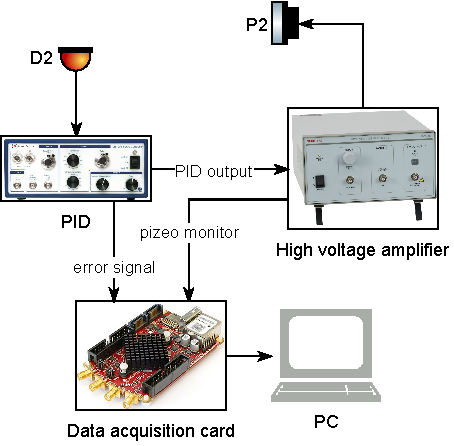
\includegraphics[width=0.4\linewidth]{fig_3_optical_path_370_Interferometer_devices.pdf}}
    \subcaptionbox{The circuit diagram.}
    {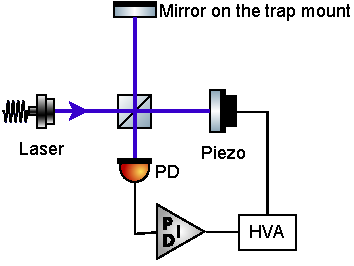
\includegraphics[width=0.4\linewidth]{fig_3_optical_path_370_Interferometer_diagram.pdf}}
    \caption{The circuit diagram of the Michelson interferometer.}
\end{figure}

A Michelson interferometer-based measurement solution requires a very stable laser source. Or rather the measurement error is directly related to the jitter of the laser source. This is because we do not currently use a solution similar to the Mach-Zehnder interferometer, so the PID can only be locked to the rising edge of the fringe of the signal, and the addition of a modulation module would reduce the interference caused by laser source jitter, i.e. improve the signal-to-noise ratio. Experimentally, the coherence length of a single-frequency laser should be much greater than 1 m, and the power and polarisation jitter should ideally be less than 1\%, and at worst no more than 5\%. Fortunately, the 370 nm laser (C10) we used meets these requirements and can be used as the laser source for the laser interferometer, thus reducing the cost of building the instrument ourselves. One arm of the interferometer comes from the return laser from the reflector on the trap holder and the other arm comes from the return laser from the reflector fixed to the optical table (P2; PA44LEW Throlabs), so we can measure the change in the optical range of the trap relative to the optical table. The interferometric laser is directed at the photodiode and the photocurrent is passed through the transimpedance amplifier to generate an interference voltage signal. The error signal generated by the PID module is then output to a high voltage amplifier, which generates a voltage signal to drive the piezoelectric ceramic on the optical table reflector. This creates a phase-locked loop and by reading the value of the voltage signal from the piezoelectric ceramic we can determine the change in the optical path of the reflector on the trap holder. The feedback bandwidth of this loop is approximately 1 kHz, which is limited by the bandwidth and linear operating range of the piezoelectric ceramic. We have increased the feedback bandwidth of the phase-locked loop by choosing to use a high bandwidth piezoelectric ceramic and a small mass of reflector as a load on the piezoelectric ceramic.

\subsection{High-precision long-term vibration measurement}

\begin{figure}
    \centering
    \subcaptionbox{Interferometer with high stability.}
    {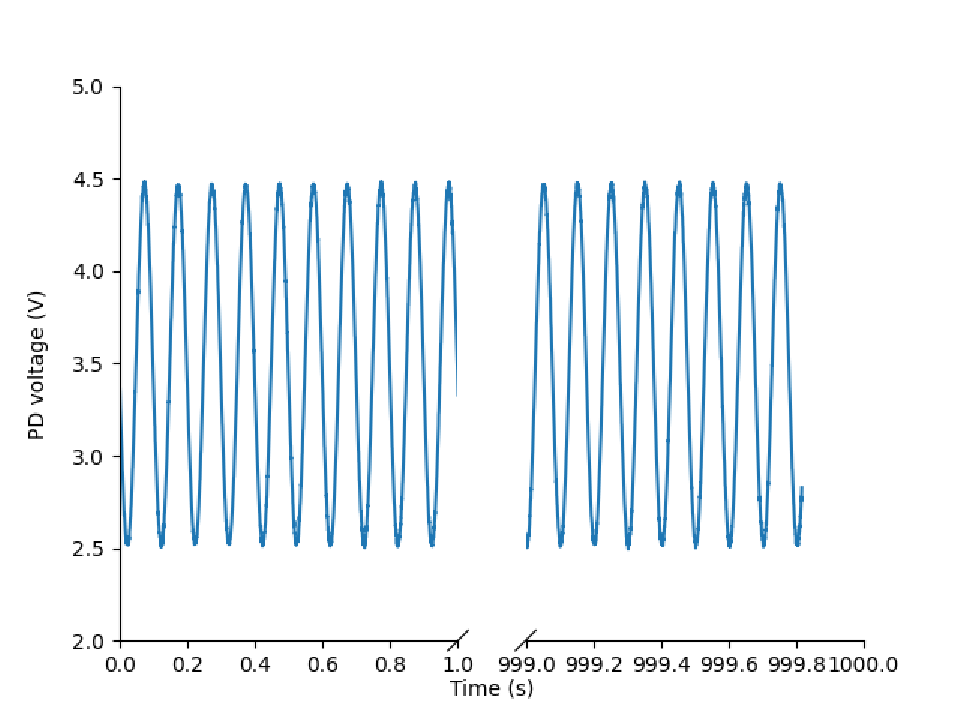
\includegraphics[width=0.4\linewidth]{fig_4_vibration_calibration_interferometer_with_high_stability.pdf}}
    \subcaptionbox{Interferometer with high precision.}
    {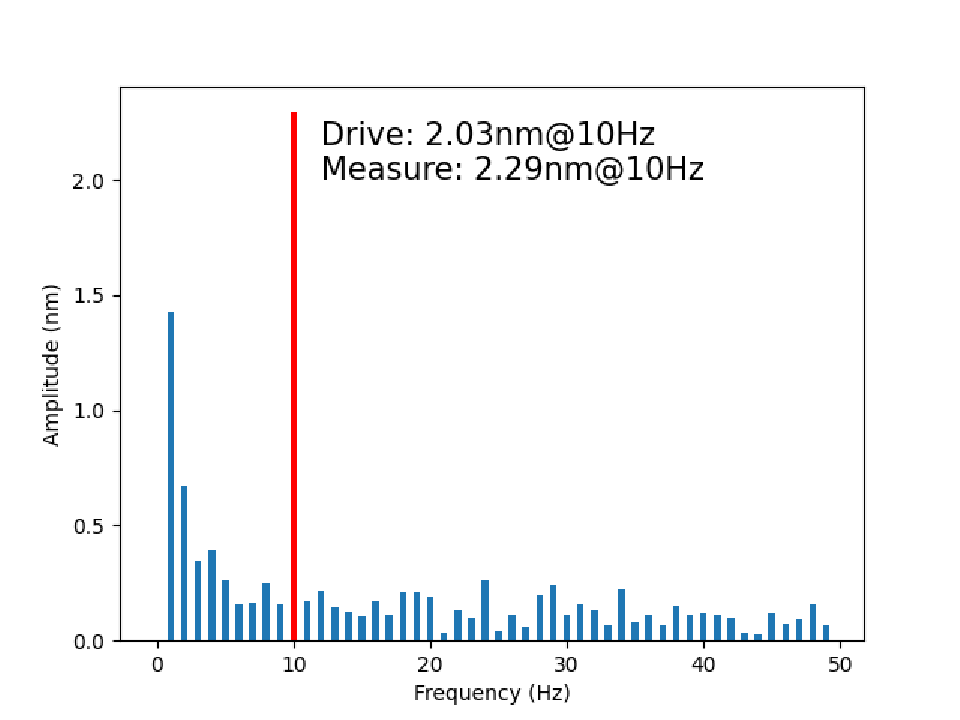
\includegraphics[width=0.4\linewidth]{fig_4_vibration_calibration_interferometer_with_high_precision.pdf}}
    \caption{Interferometer with high stability and precision.}
    \label{fig:fig_4_vibration_calibration_interferometer}
\end{figure}

Before a mature cryostat is developed, we usually debug some experimental phenomena and experimental parameters repeatedly in our experiments. These problems due to the immaturity of the cryostat can arise from mechanical design, optical errors and electrical noise. We usually analyse these problems by comparing a cryogenic trap system with a room-temperature trap system, which is simpler in structure and therefore more stable. So a stable cryostat can greatly guarantee the rapid forward movement of our experimental process. Some stability may be necessary, such as vibrations in the laser manipulation sequence, which may affect the quantum gate fidelity, and long-term drift, which may affect the possibility of individual addressing. It is therefore necessary to experimentally measure the trapped ions with respect to the laser's optical path precisely and over a long period of time to achieve passive stabilisation of the various parameters of the cryostat. Fig~\ref{fig:fig_4_vibration_calibration_interferometer} proves that this interferometer is very stable and the measurement result is precise.

Before carrying out the measurements, I calibrated the instrument. The wavelength of the laser coming out of the single-mode polarisation-maintain fibre (C10) was 370 nm, and I first checked the stability of the power and polarisation of the light coming out of the fibre by connecting it to a power meter and a polarisation analyser respectively. After confirming the stability of the laser source, I also checked the long-term stability of the interference signal, mainly by measuring the stability of the maximum and minimum values of the interference signal. I used epoxy glue to glue the reflector, piezoelectric ceramic and mirror mount together. Although the product manual for piezoelectric ceramics gives a relationship between displacement and voltage, in practice I have found that the linearity of these mirrors varies considerably from one production to the next, and in some cases the linearity changes after a few months. It is therefore necessary to calibrate the relationship between the displacement of the mirror and the voltage, as shown in Fig~\ref{fig:fig_4_vibration_calabration_pzt}. I use a flipper mirror (N2) to change one arm of the interferometer from the chamber to another mirror on the optical table, as the change in the interference signal at this point is so small that it can be assumed that there is no additional vibration. I applied a drive signal to the piezoelectric ceramic of the reflector to be calibrated and could see the interferometric signal oscillate.

\begin{figure}
    \centering
    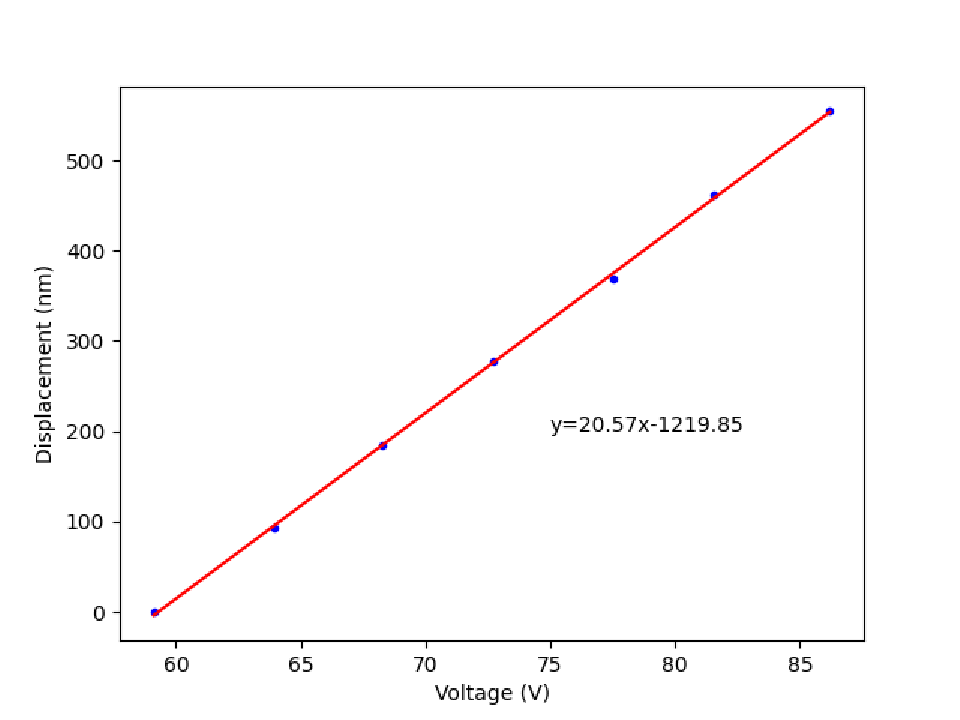
\includegraphics[width=0.4\linewidth]{fig_4_vibration_calabration_pzt.pdf}
    \caption{Voltage-to-displacement conversion of the piezo.}
    \label{fig:fig_4_vibration_calabration_pzt}
\end{figure}

The relationship between the driving voltage and the interference signal deviates from sinusoidal oscillations because the driving relationship is not linear and the change in the angle of the mirror during the application of the driving signal causes a consequent change in the contrast of the interference signal. I calculated the optical path by selecting the eigenpoints of the interferometric maximum and minimum values. In the end, I can calculate the linear coefficients of the driving voltage and displacement for each manufactured reflector. In principle I could measure the vibration signal of the trap immediately, but to ensure that the measurement was correct I carried out a simulation experiment. By applying a drive signal to the mirrors of the other arm of the interferometer, the linear coefficients of voltage and displacement of each mirror were of course calibrated, and then the drive signal of the measured mirrors was read out. A comparison of these two signals gives the measurement accuracy.

\subsection{Minimize vibration of the cryostat}

In our laboratory, the vibration of the optical elements on the floating optical platform is around a few tens of nm, and our ultimate goal is to reduce the vibration of the cryostat to this order of magnitude. In our initial cryostat setup, the vibrations were in the order of a few hundred nm, half of which stemmed from the instability of the internal structure of the chamber and the other half from the vibrations caused by the cold head. Since vibrations of several hundred nm were also measured when the chiller was switched off, we decided to reinforce the internal structure of the chamber. In addition to the vibrations over a short period of time, the ions produce a translation of 1-10 $\mu$m during the process of doing the experiment, which indicates a long drift inside the chamber in response to environmental changes, as evidenced by the interferometer measurements. We first modified the support point in the 4 K region of the chamber.

\begin{figure}
    \centering
    \subcaptionbox{Vibration in the time domain.}
    {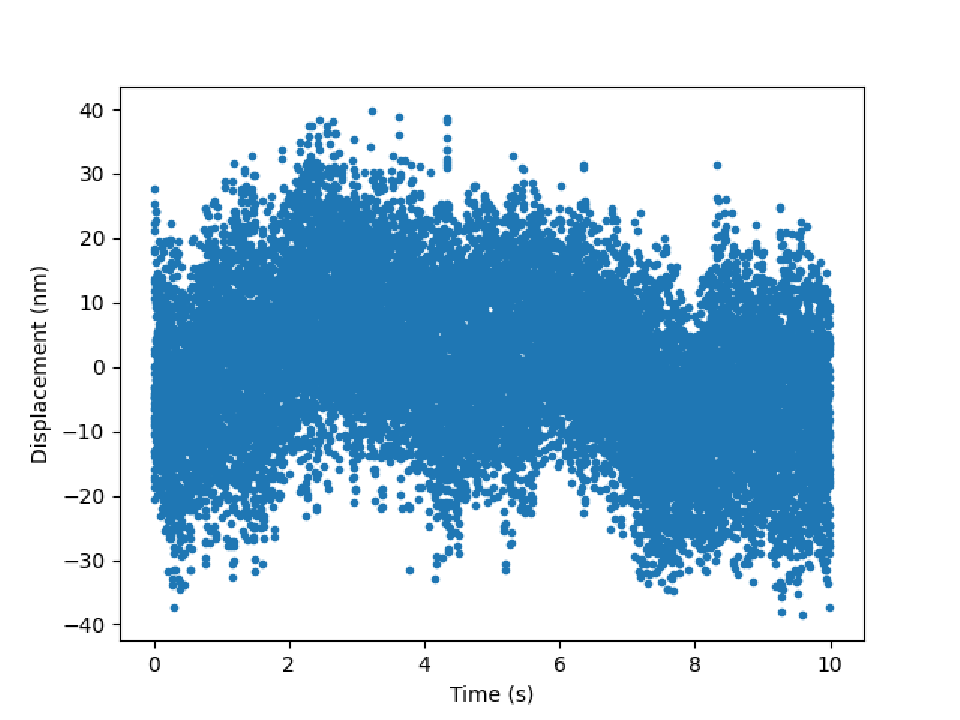
\includegraphics[width=0.4\linewidth]{fig_4_vibration_HYQ.pdf}}
    \subcaptionbox{Vibration in the frequency domain.}
    {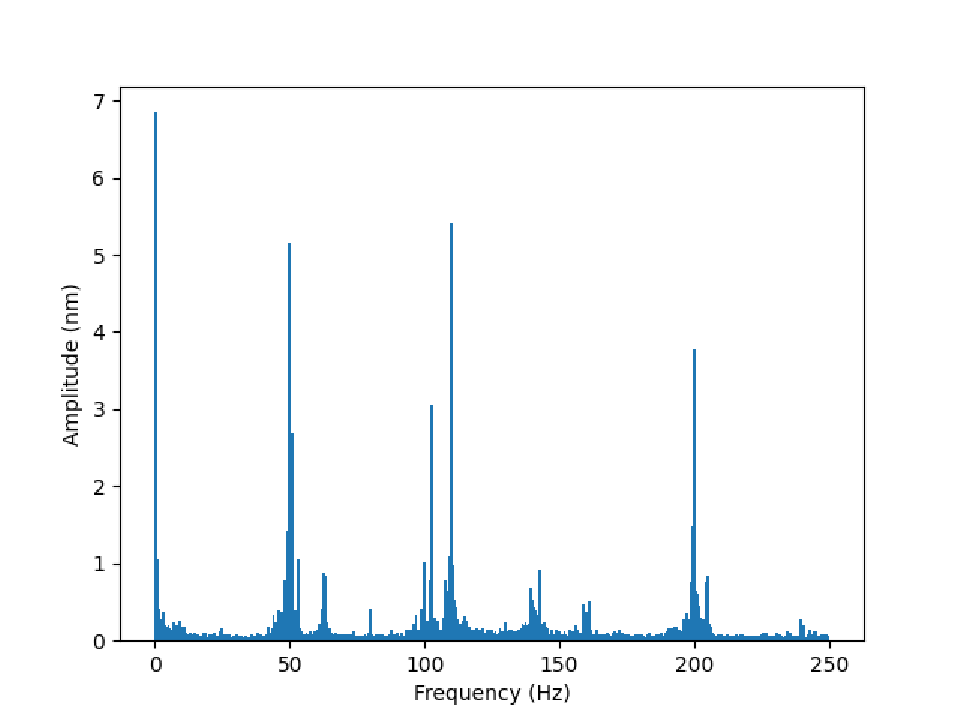
\includegraphics[width=0.4\linewidth]{fig_4_vibration_HYQ_fft.pdf}}
    \subcaptionbox{Long-term vibration.}
    {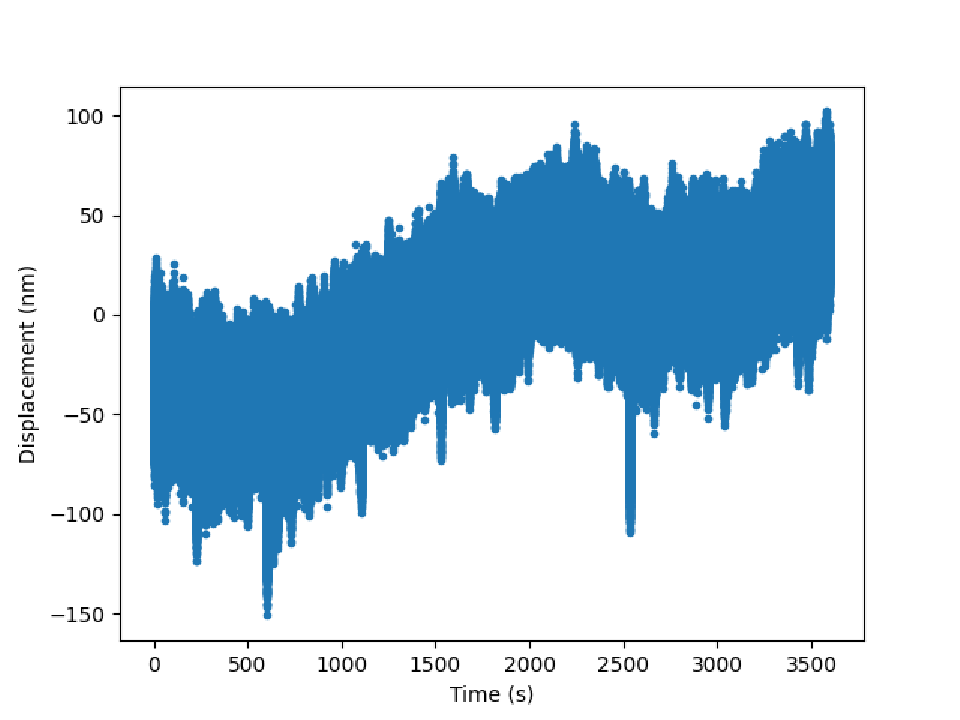
\includegraphics[width=0.4\linewidth]{fig_4_vibration_HYQ_longterm.pdf}}
    \subcaptionbox{Allan variance of long-term vibration.}
    {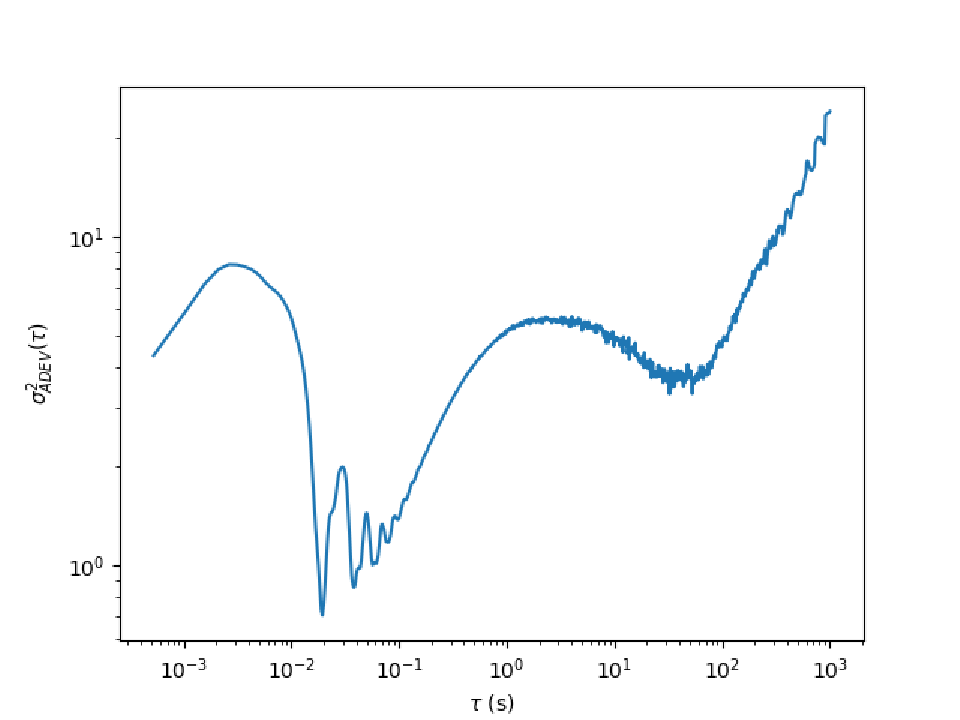
\includegraphics[width=0.4\linewidth]{fig_4_vibration_HYQ_longterm_allan.pdf}}
    \caption{Vibration in the horizontal plane of the cryostat after optimization.}
    \label{fig:fig_4_vibration_HYQ}
\end{figure}

Previously the support passed through the whole of the exchange gas region and was therefore subject to long drift due to changes in the environment of the exchange gas region. We have now moved the support to the 300 K region and shortened the support material. Although we will lose some refrigeration capacity, we have solved the problem of long drift. We found that the suspension design did not allow enough support points for the 4 K shield and 40 K shield, so we added PEEK connectors to the bottom of the shield. By optimising the structural design of the chamber \cite{RN261}, we managed to solve the vibration and long drift problems. Fig~\ref{fig:fig_4_vibration_HYQ} shows the vibration signal of the optimised cryostat.



\section {Obtain impedance match of helical resonator}

If the RF voltage is applied directly from the RF amplifier to the ion trap, the following problems may be caused. An impedance mismatch between the RF amplifier and the ion trap will cause the RF signal to be reflected from the ion trap, resulting in power dissipation in the output impedance of the RF amplifier. The RF amplifier will also input noise into the ion trap, which may lead to heating of the ions \cite{RN360,RN162,RN276,RN135}. So we connect the output of the RF amplifier to a helical resonator. Due to the damping effect of the output impedance of the RF amplifier, connecting the helical resonator directly to the RF amplifier will reduce the quality factor of the spiral resonator, so this connection can be achieved by capacitive or inductive coupling, thus decoupling the helical resonator from the resistive output impedance of the RF amplifier, as well as giving the spiral resonator a high quality factor. This technique allows the impedance of the ion trap and the RF amplifier to be matched by varying the coupling, thereby reducing the reflected power and therefore the output power of the RF amplifier when the voltage required to generate the ion trap is reduced. Passing the output of the RF amplifier through a resonator allows the noise to be filtered and its contribution to the ion heating to be reduced to the greatest extent possible due to the high quality factor and narrow bandwidth of the resonator \cite{RN337,RN342,RN340,RN330,RN332}.

\begin{figure}
    \centering
    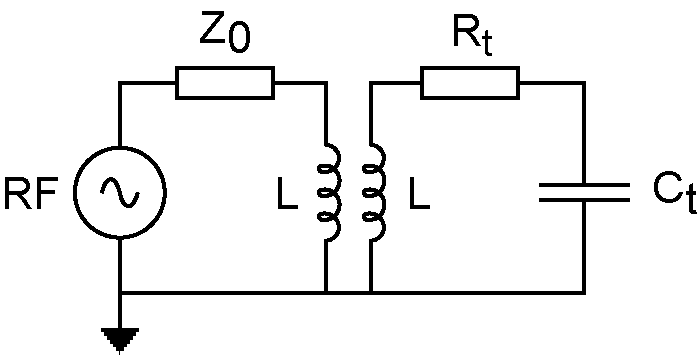
\includegraphics[width=0.8\linewidth]{fig_4_impedance_match_circuit_diagram_a.pdf}
    \caption{Circuit diagram of the helical resonator.}
    \label{fig:fig_4_impedance_match_circuit_diagram_a}
\end{figure}

This shows that it is very important to obtain a high quality factor and to achieve impedance matching for the blade trap. For the room-temperature trap, we can feed the RF signal into the blade trap via feedthrough after the vacuum chamber has been established, so we can assemble and test the helical resonator that generates the RF signal on the optical table. For the cryogenic trap we need to place the helical resonator inside the vacuum chamber. This reduces the circuit resistance to obtain a high quality factor, maintains the relative temperature stability of the helical resonator and the blade trap, and reduces electrical noise by reducing the circuit length and temperature.

\begin{figure}
    \centering
    \subcaptionbox{\label{fig:fig_4_impedance_match_circuit_diagram_b}}
    {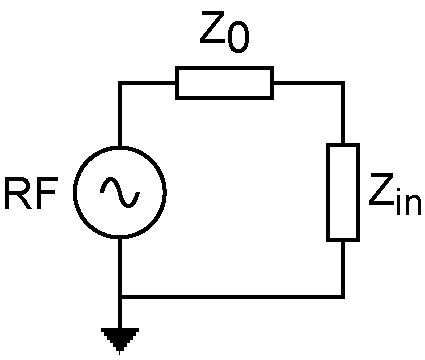
\includegraphics[width=0.5\linewidth]{fig_4_impedance_match_circuit_diagram_b.pdf}}
    \subcaptionbox{\label{fig:fig_4_impedance_match_circuit_diagram_c}}
    {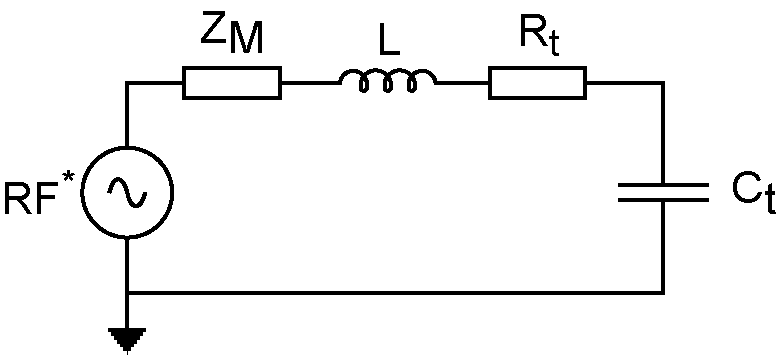
\includegraphics[width=0.7\linewidth]{fig_4_impedance_match_circuit_diagram_c.pdf}}
    \caption{Simplified circuit diagrams of the helical resonator.}
    \label{fig:fig_4_impedance_match_circuit_diagram}
\end{figure}

At the same time the quality factor is very much improved at low temperatures due to the reduced resistance compared to a room-temperature trap. However, the impedance matching is disrupted due to the reduced resistance at low temperatures and we need to find a way to achieve impedance matching at low temperatures. The impedance matching parameters can be found using the dichotomous method by repeated warm-up and cool-down test operations, but a single warm-up operation lasting at least 2 days is too cumbersome. By modelling the RF system and measuring the system parameters in a single run, we can find a convenient way to adjust the impedance matching.

We can indirectly measure the loaded quality factor of the helical resonator by using the ${S}_{11}$ parameter measured by the vector network analyzer.
\begin{equation}
    Q_L = \frac{Q_U}{1 + \kappa},\ \kappa =\\
    \begin{cases}
        \mathrm{SWR},     & \text{over couple}     \\
        1,                & \text{critical couple} \\
        1 / \mathrm{SWR}, & \text{under couple}    \\
    \end{cases}
    ,\ \mathrm{SWR} = \frac{1 + |\Gamma|}{1 - |\Gamma|},
\end{equation}
where $Q_L$ is the loaded quality factor, $Q_I$ is the unloaded quality factor, $\kappa$ is the coupling coefficient of the resonator, SWR is the standing wave ratio, $\Gamma$ is a complex number that describes both the magnitude and the phase shift of the reflection.

Fig~\ref{fig:fig_4_impedance_match_circuit_diagram} shows the circuit diagram of the helical resonator. $Z_0$ is the internal resistance of the RF signal source, $Z_0$ = 50 $\Omega$, L is the inductance of the antenna and helical copper wire, $R_t$ is the AC resistance of the trap, $C_t$ is the equivalent capacitance of the trap, $Z_{in}$ is the equivalent impedance of the trap, and $Z_M$ is the equivalent impedance of the mutual induction.
\begin{equation}
    \begin{aligned}
        Z_{in} & =i \omega L+\frac{(k \omega L)^2}{i \omega L+R_t+\frac{1}{i \omega C}}, \\
        Z_M    & =\frac{k^2 \omega^2 L^2}{i \omega L+Z_0},
    \end{aligned}
\end{equation}
where k is the coefficient of mutual induction. When the circuit is resonant, the imaginary part of the total impedance in Fig~\ref{fig:fig_4_impedance_match_circuit_diagram_c} is 0. The frequency at this point is,
\begin{equation}
    \omega=\frac{Z_0}{L} \sqrt{\frac{\alpha-1+\sqrt{(\alpha+1)^2-4 \alpha k^2}}{2\left(1-k^2\right)}},\ \\
    \alpha=\frac{L}{Z_0^2 C}.
\end{equation}

When we obtain impedance matching by adjusting the antenna coupling $k$, $Z_{in} = Z_0$ in Fig~\ref{fig:fig_4_impedance_match_circuit_diagram_b},
\begin{equation}
    \begin{aligned}
        k      & =\sqrt{\frac{R_t}{Z_0}+\frac{C}{L} R_t\left(Z_0-R_t\right)}, \\
        \omega & =\sqrt{\frac{Z_0}{L C(Z_0-R_t)}},
    \end{aligned}
\end{equation}

We can now answer the question as to why the empirical operation of pulling a helical resonator antenna out to impedance mismatch at room temperature is valid. During the cool-down process, $R_t$ decreases continuously, so that $k$ is smaller at low temperatures than at room temperature. The only experimental parameter that we have not been able to obtain so far is $R_t$ at low temperature, which is difficult to predict theoretically, so we can derive this from a single cool-down progress.